% ============================================================
%  CS3401 – Chapter 6: Dynamic Programming
% ============================================================
\documentclass[aspectratio=169]{beamer}
% ============================================================
%  CS3401 – Algorithm Design and Analysis
%  Shared Beamer Theme (input this file in every chapter)
%  Prince Sattam Bin Abdulaziz University – CCES
% ============================================================

% ---------- PACKAGES ----------------------------------------
\usepackage[utf8]{inputenc}
\usepackage[T1]{fontenc}
\usepackage{lmodern}
\usepackage{amsmath,amssymb,amsthm}
\usepackage{tikz}
\usepackage{pgfplots}
\usepackage{booktabs}
\usepackage{xcolor}
\usepackage{graphicx}
\usepackage{listings}
\usepackage[normalem]{ulem}
\usepackage{algorithm}
\usepackage{algpseudocode}
\usepackage{multicol}
\usepackage{array}
\usepackage{colortbl}
\usepackage{tabularx}
\usepackage{makecell}

\usetikzlibrary{
  arrows.meta, shapes.geometric, shapes.symbols,
  positioning, calc, fit, backgrounds,
  decorations.pathreplacing, decorations.markings,
  matrix, chains, trees
}
\pgfplotsset{compat=1.18}

% ---------- COLOR PALETTE -----------------------------------
\definecolor{PrimaryDark}{RGB}{10,72,92}
\definecolor{PrimaryMid}{RGB}{18,114,145}
\definecolor{PrimaryLight}{RGB}{185,224,238}
\definecolor{AccentOrange}{RGB}{210,103,22}
\definecolor{AccentYellow}{RGB}{252,198,40}
\definecolor{SuccessGreen}{RGB}{32,122,66}
\definecolor{AlertRed}{RGB}{172,46,46}
\definecolor{CodeBg}{RGB}{244,246,250}
\definecolor{DarkText}{RGB}{28,32,40}
\definecolor{LightRule}{RGB}{210,225,232}
\tikzset{processstep/.style={draw=PrimaryMid, fill=PrimaryLight!35, rounded corners=2pt,
  align=center, minimum width=4.2cm, minimum height=0.55cm, font=\small}}

% ---------- BEAMER SETTINGS ---------------------------------
\setbeamertemplate{navigation symbols}{}
\setbeamertemplate{caption}[numbered]

% Fonts
\setbeamerfont{normal text}{size=\small}
\setbeamerfont{title}{series=\bfseries,size=\LARGE}
\setbeamerfont{subtitle}{series=\normalfont,size=\large}
\setbeamerfont{frametitle}{series=\bfseries,size=\large}
\setbeamerfont{framesubtitle}{series=\normalfont,size=\small}
\setbeamerfont{block title}{series=\bfseries,size=\normalsize}
\setbeamerfont{footline}{size=\tiny}
\addtobeamertemplate{frame begin}{\small\enlargethispage{1cm}}{}
\setlength{\tabcolsep}{2pt}

% Colors
\setbeamercolor{normal text}{fg=DarkText,bg=white}
\setbeamercolor{frametitle}{bg=PrimaryDark,fg=white}
\setbeamercolor{title}{fg=white}
\setbeamercolor{subtitle}{fg=PrimaryLight}
\setbeamercolor{author}{fg=white}
\setbeamercolor{date}{fg=PrimaryLight}
\setbeamercolor{institute}{fg=PrimaryLight}
\setbeamercolor{block title}{bg=PrimaryMid,fg=white}
\setbeamercolor{block body}{bg=PrimaryLight!35,fg=DarkText}
\setbeamercolor{block title alerted}{bg=AlertRed,fg=white}
\setbeamercolor{block body alerted}{bg=AlertRed!12,fg=DarkText}
\setbeamercolor{block title example}{bg=SuccessGreen,fg=white}
\setbeamercolor{block body example}{bg=SuccessGreen!12,fg=DarkText}
\setbeamercolor{itemize item}{fg=PrimaryMid}
\setbeamercolor{itemize subitem}{fg=AccentOrange}
\setbeamercolor{enumerate item}{fg=PrimaryMid}
\setbeamercolor{enumerate subitem}{fg=AccentOrange}
\setbeamercolor{alerted text}{fg=AlertRed}
\setbeamercolor{structure}{fg=PrimaryMid}
\setbeamercolor{section in toc}{fg=PrimaryDark}
\setbeamercolor{section in toc shaded}{fg=PrimaryDark}
% override Beamer's transparency-based shading so TOC entries stay fully visible
\setbeamertemplate{section in toc shaded}{\inserttocsection\par}
\setbeamercolor{subsection in toc}{fg=PrimaryMid}
\setbeamercolor{footer rule}{bg=LightRule}

% Item symbols
\setbeamertemplate{itemize item}{%
  \scriptsize\raise1.5pt\hbox{\color{PrimaryMid}$\blacktriangleright$}}
\setbeamertemplate{itemize subitem}{%
  \scriptsize\raise1pt\hbox{\color{AccentOrange}$\bullet$}}
\setbeamertemplate{itemize subsubitem}{%
  \scriptsize\raise1pt\hbox{\color{PrimaryDark}$\circ$}}
\setbeamertemplate{enumerate item}{%
  \color{PrimaryMid}\textbf{\insertenumlabel.}}

% Frame title
\makeatletter
\setbeamertemplate{frametitle}{%
  \nointerlineskip
  \begin{beamercolorbox}[wd=\paperwidth,ht=2.4em,dp=0.9em,%
                         leftskip=1.2em,rightskip=1.2em]{frametitle}
    \usebeamerfont{frametitle}\insertframetitle\strut
    \ifx\insertframesubtitle\@empty\else
      \hspace{0.6em}\textcolor{PrimaryLight!80}{\footnotesize|}\hspace{0.4em}%
      {\usebeamerfont{framesubtitle}\textcolor{PrimaryLight}\insertframesubtitle}%
    \fi
  \end{beamercolorbox}
  \nointerlineskip
  \begin{beamercolorbox}[wd=\paperwidth,ht=0.3pt,dp=0pt]{structure}
  \end{beamercolorbox}
}
\makeatother

% Footer
\setbeamertemplate{footline}{%
  \begin{beamercolorbox}[wd=\paperwidth,ht=0.4pt,dp=0pt]{footer rule}{}
  \end{beamercolorbox}
  \leavevmode
  \hbox{%
    \begin{beamercolorbox}[wd=0.60\paperwidth,ht=1.8em,dp=0.6em,leftskip=1em]{normal text}%
      \textcolor{PrimaryDark}{\tiny\textbf{CS3401} \textendash{} Algorithm Design \& Analysis%
        \quad\textbar\quad CCES, PSAU}%
    \end{beamercolorbox}%
    \begin{beamercolorbox}[wd=0.40\paperwidth,ht=1.8em,dp=0.6em,rightskip=1em,right]{normal text}%
      \textcolor{PrimaryDark}{\tiny\insertshorttitle%
        \quad\textbar\quad\insertframenumber\,/\,\inserttotalframenumber}%
    \end{beamercolorbox}%
  }%
}

% Title page
\setbeamertemplate{title page}{%
  
\begin{tikzpicture}[remember picture,overlay]
    \fill[PrimaryDark](current page.north west) rectangle (current page.south east);
    \fill[PrimaryMid,opacity=0.45]
      ([shift={(2.5cm,-2.5cm)}]current page.north east) circle(5.5cm);
    \fill[AccentOrange,opacity=0.10]
      ([shift={(-1.5cm,2.0cm)}]current page.south west) circle(4.2cm);
    \draw[white,opacity=0.08,line width=40pt]
      ([shift={(0cm,-0.5cm)}]current page.north west)
      to[out=-30,in=210]
      ([shift={(0cm,0.5cm)}]current page.south east);
  \end{tikzpicture}%
  \vspace{0.7cm}
  \begin{center}
    {\tiny\textcolor{PrimaryLight}{\textbf{CCES} \textendash{}
      College of Computer Engineering and Sciences}}\\[0.2em]
    {\tiny\textcolor{PrimaryLight}{Prince Sattam Bin Abdulaziz University}}\\[1.2em]
    {\footnotesize\textcolor{AccentYellow}{\textbf{CS3401 \textendash{} Algorithm Design and Analysis}}}\\[1.5em]
    \textcolor{PrimaryMid}{\rule{0.55\textwidth}{0.6pt}}\\[0.9em]
    {\Large\usebeamerfont{title}\textcolor{white}{\inserttitle}}\\[0.4em]
    {\small\usebeamerfont{subtitle}\textcolor{PrimaryLight}{\insertsubtitle}}\\[0.7em]
    \textcolor{PrimaryMid}{\rule{0.55\textwidth}{0.6pt}}\\[1.2em]
    {\footnotesize\textcolor{PrimaryLight}{\insertdate}}\\[0.6em]
    % Instructors row
    \begin{tikzpicture}[baseline=(current bounding box.center)]
      % Dr. Khalil – rounded photo
      \begin{scope}
        \clip (-3.2,0) circle (0.58cm);
        \node at (-3.2,0)
          {
\includegraphics[width=1.16cm,height=1.16cm,keepaspectratio=false]{khalil}};
      \end{scope}
      \draw[white,line width=0.9pt] (-3.2,0) circle (0.58cm);
      \node[text=white,font=\scriptsize\bfseries,anchor=west] at (-2.54,0)
        {Dr.\ Khalil Chebil};
      % Dr. Esraa – placeholder circle
      \draw[white,line width=0.9pt] (1.2,0) circle (0.58cm);
      \node[text=PrimaryLight,font=\normalsize\bfseries] at (1.2,0) {E};
      \node[text=white,font=\scriptsize\bfseries,anchor=west] at (1.86,0)
        {Dr.\ Esraa};
    \end{tikzpicture}
  \end{center}%
}

% Auto section-divider slide — background set via Beamer color system for reliability
\AtBeginSection[]{%
  {%
    \setbeamercolor{background canvas}{bg=PrimaryDark}%
    \begin{frame}[plain,noframenumbering]
      \begin{tikzpicture}[remember picture,overlay]
        \fill[PrimaryMid,opacity=0.35]
          ([shift={(0cm,-1.5cm)}]current page.north) circle(6.5cm);
        \node[text=white,opacity=0.06,font=\fontsize{120}{120}\bfseries]
          at ([shift={(-1cm,0cm)}]current page.center)
          {\insertsectionnumber};
      \end{tikzpicture}
      \vfill
      \begin{center}
        {\large\textcolor{AccentYellow}{\textbf{Section \insertsectionnumber}}}\\[0.6em]
        {\LARGE\textcolor{white}{\textbf{\insertsectionhead}}}
      \end{center}
      \vfill
    \end{frame}
  }%
}

% ---------- LISTINGS STYLE ----------------------------------
\lstset{
  basicstyle=\ttfamily\footnotesize,
  backgroundcolor=\color{CodeBg},
  keywordstyle=\color{PrimaryMid}\bfseries,
  commentstyle=\color{SuccessGreen}\itshape,
  stringstyle=\color{AccentOrange},
  numberstyle=\tiny\color{gray!70},
  frame=tb,
  framerule=0.5pt,
  rulecolor=\color{PrimaryLight},
  numbers=left,
  numbersep=6pt,
  showstringspaces=false,
  breaklines=true,
  tabsize=2,
  xleftmargin=1.8em,
  framexleftmargin=1.8em,
  captionpos=b,
  language=Java,
  morekeywords={var,let,const}
}

% ---------- PSEUDOCODE STYLE --------------------------------
\algrenewcommand\algorithmicprocedure{\textbf{Algorithm}}
\algrenewcommand\algorithmicfunction{\textbf{Function}}
\algrenewcommand\algorithmicif{\textbf{if}}
\algrenewcommand\algorithmicelse{\textbf{else}}
\algrenewcommand\algorithmicthen{\textbf{then}}
\algrenewcommand\algorithmicwhile{\textbf{while}}
\algrenewcommand\algorithmicfor{\textbf{for}}
\algrenewcommand\algorithmicforall{\textbf{for all}}
\algrenewcommand\algorithmicreturn{\textbf{return}}
\algrenewcommand\algorithmicend{\textbf{end}}
\algrenewcommand\algorithmicdo{}
\algrenewcommand\algorithmicrequire{\textbf{Input:}}
\algrenewcommand\algorithmicensure{\textbf{Output:}}

% ---------- CUSTOM COMMANDS ---------------------------------
\newcommand{\bigO}[1]{$\mathcal{O}(#1)$}
\newcommand{\bigTheta}[1]{$\Theta(#1)$}
\newcommand{\bigOmega}[1]{$\Omega(#1)$}
\newcommand{\highlight}[1]{\colorbox{AccentYellow!55}{\strut #1}}
\newcommand{\important}[1]{\textcolor{AlertRed}{\bfseries #1}}
\newcommand{\keyword}[1]{\textcolor{PrimaryMid}{\bfseries #1}}
\newcommand{\concept}[1]{\textcolor{AccentOrange}{\bfseries #1}}

% Colored table column types
\newcolumntype{H}{>{\columncolor{PrimaryDark}\color{white}\bfseries\centering\arraybackslash}m{2.5cm}}
\newcolumntype{Z}{>{\columncolor{PrimaryLight!40}\centering\arraybackslash}m{2cm}}

% Reference boxes
\newcommand{\refbox}[1]{%
  \begin{beamercolorbox}[rounded=true,shadow=false,leftskip=0.5em,rightskip=0.5em,%
                          ht=1.6em,dp=0.5em]{block title}
    \small\textit{Reference:} #1
  \end{beamercolorbox}%
}

% Inline complexity tag
\newcommand{\ctag}[1]{%
  \hfill\tikz[baseline]{\node[fill=AlertRed,text=white,rounded corners=2pt,
    font=\bfseries\scriptsize,inner sep=2pt,outer sep=0pt]{$\mathcal{O}(#1)$};}%
}


\title[Ch.\,6 -- Dynamic Programming]{Chapter 6}
\subtitle{Dynamic Programming}
\date{Academic Year 2026\,--\,2027}

\begin{document}

\begin{frame}[plain]\titlepage\end{frame}
\begin{frame}[shrink=20]{Chapter Overview}
  \begin{center}
    \begin{minipage}{0.85\textwidth}
      \tableofcontents[hideallsubsections,sectionstyle=show/shaded]
    \end{minipage}
  \end{center}
\end{frame}

% ============================================================
\section{Introduction}
% ============================================================

\begin{frame}[shrink=12]{The Fibonacci Trap}
  \begin{columns}[T]
    \column{0.55\textwidth}
      \textbf{Naive recursive Fibonacci:}
      \begin{algorithmic}[1]
        \State $\text{fib}(n)$:
        \If{$n\leq 1$} \Return $n$ \EndIf
        \State \Return $\text{fib}(n{-}1) + \text{fib}(n{-}2)$
      \end{algorithmic}
      \vspace{0.3em}
      Recurrence: $T(n) = T(n{-}1) + T(n{-}2) + \mathcal{O}(1)$
      \[
        T(n) \in \Theta\!\left(\varphi^n\right),\;\varphi\approx 1.618
      \]
      \textbf{Exponential time} — fib(50) makes $\approx 10^{10}$ calls!

      \vspace{0.3em}
      \begin{alertblock}{Root cause}
        The same sub-problem (e.g.\ fib(10)) is computed
        \emph{exponentially many times}.
      \end{alertblock}
    \column{0.40\textwidth}
      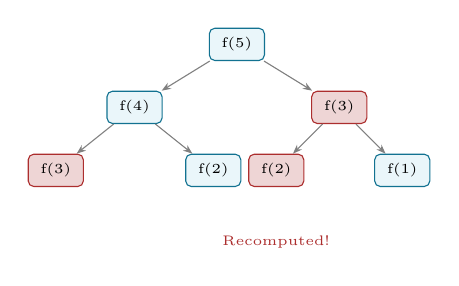
\begin{tikzpicture}[
        nd/.style={draw=PrimaryMid,fill=PrimaryLight!30,rounded corners=2pt,
                   font=\tiny,minimum width=0.7cm,minimum height=0.4cm},
        dup/.style={draw=AlertRed,fill=AlertRed!20,rounded corners=2pt,
                    font=\tiny,minimum width=0.7cm,minimum height=0.4cm},
        arr/.style={-{Stealth[scale=0.7]},gray}
      ]
        \node[nd] (f5) at (2.5,3.5) {f(5)};
        \node[nd] (f4l) at (1.2,2.7) {f(4)};
        \node[dup] (f3l) at (3.8,2.7) {\alert{f(3)}};
        \node[dup] (f3a) at (0.2,1.9) {\alert{f(3)}};
        \node[nd] (f2l) at (2.2,1.9) {f(2)};
        \node[dup] (f2a) at (3.0,1.9) {\alert{f(2)}};
        \node[nd] (f1a) at (4.6,1.9) {f(1)};
        \draw[arr] (f5)--(f4l); \draw[arr] (f5)--(f3l);
        \draw[arr] (f4l)--(f3a); \draw[arr] (f4l)--(f2l);
        \draw[arr] (f3l)--(f2a); \draw[arr] (f3l)--(f1a);
        \node[font=\tiny,text=AlertRed,below=0.5cm of f2a]
          {Recomputed!};
      \end{tikzpicture}
  \end{columns}
\end{frame}

\begin{frame}[shrink=12]{Dynamic Programming — The Fix}
  \begin{block}{Dynamic Programming (DP)}
    An algorithm design technique for solving problems with
    \keyword{overlapping sub-problems} by computing each sub-problem
    \emph{once} and storing the result in a table.
    ``Programming'' here means \emph{planning} (not coding).
  \end{block}
  \vspace{0.4em}
  \begin{columns}[T]
    \column{0.50\textwidth}
      \textbf{Two approaches:}
      \begin{itemize}
        \item \concept{Tabulation (bottom-up)}: fill table from smallest
              sub-problems up to the target; iterative; no recursion overhead
        \item \concept{Memoisation (top-down)}: recursive, but cache
              each result; compute only what is needed
      \end{itemize}
      \vspace{0.3em}
      \textbf{Fibonacci with DP:}\\
      Fill table $F[0..n]$ left to right: $F[i] = F[i{-}1] + F[i{-}2]$\\
      Time: $\Theta(n)$ \quad Space: $\Theta(n)$ (or $\mathcal{O}(1)$ if only last two kept)
    \column{0.45\textwidth}
      \begin{exampleblock}{Key conditions for DP}
        \begin{enumerate}
          \item \textbf{Optimal substructure}: optimal solution
                is built from optimal solutions of sub-problems
          \item \textbf{Overlapping sub-problems}: sub-problems
                share common sub-sub-problems (unlike D\&C)
        \end{enumerate}
      \end{exampleblock}
      \vspace{0.3em}
      \textbf{DP vs.\ Divide \& Conquer:}\\
      D\&C splits into \emph{independent} sub-problems.\\
      DP handles \emph{overlapping} ones.
  \end{columns}
\end{frame}

% ============================================================
\section{Coin-Row Problem}
% ============================================================

\begin{frame}[shrink=12]{Coin-Row Problem (House Robber)}
  \begin{block}{Problem}
    Given a row of $n$ coins with values $c_1, c_2, \ldots, c_n$,
    pick up the maximum total value subject to: \emph{no two adjacent
    coins may be selected}.
  \end{block}
  \vspace{0.3em}
  \begin{columns}[T]
    \column{0.55\textwidth}
      \textbf{Recurrence:} Let $F(i)$ = max value from coins $1..i$:
      \[
        F(i) = \max\bigl\{c_i + F(i-2),\; F(i-1)\bigr\}
      \]
      \[
        F(0) = 0, \quad F(1) = c_1
      \]
      \textbf{Example:} $[5,\;1,\;2,\;10,\;6,\;2]$

      \vspace{0.2em}
      \begin{tabular}{c*{7}{r}}
        \toprule
        $i$ & 0 & 1 & 2 & 3 & 4 & 5 & 6 \\
        $c$ & — & 5 & 1 & 2 & 10& 6 & 2 \\
        $F$ & 0 & 5 & 5 & 7 & 15& 15& \textbf{17}\\
        \bottomrule
      \end{tabular}
    \column{0.40\textwidth}
      \textbf{Trace:}
      \begin{itemize}
        \item $F(2) = \max(1+0,5) = 5$
        \item $F(3) = \max(2+5,5) = 7$
        \item $F(4) = \max(10+5,7) = 15$
        \item $F(5) = \max(6+7,15) = 15$
        \item $F(6) = \max(2+15,15) = \highlight{17}$
      \end{itemize}
      \vspace{0.3em}
      \textbf{Optimal selection:} trace back — pick coins at positions
      1, 4, 6 (values 5, 10, 2).
      \ctag{n}
  \end{columns}
\end{frame}

% ============================================================
\section{Change-Making Problem}
% ============================================================

\begin{frame}[shrink=12]{Change-Making}
  \begin{columns}[T]
    \column{0.55\textwidth}
      \textbf{Problem:} Find the minimum number of coins from denominations
      $d_1 < d_2 < \cdots < d_m$ that sum to amount $n$.

      \vspace{0.3em}
      \textbf{Recurrence:}
      \[
        F(n) = \min_{\substack{j:\,n \geq d_j}} \bigl\{F(n - d_j)\bigr\} + 1
        \quad F(0) = 0
      \]
      \vspace{0.2em}
      \textbf{Why greedy fails:} denominations $\{1, 3, 4\}$, amount 6.\\
      Greedy: $4+1+1 = 3$ coins.\\
      DP optimal: $3+3 = \highlight{2}$ coins.
    \column{0.40\textwidth}
      \textbf{DP table for $\{1,3,4\}$, $n=6$:}
      \vspace{0.2em}

      \begin{tabular}{r*{7}{c}}
        \toprule
        $n$ & 0 & 1 & 2 & 3 & 4 & 5 & 6 \\
        \midrule
        $F$ & 0 & 1 & 2 & 1 & 1 & 2 & \textbf{2} \\
        \bottomrule
      \end{tabular}
      \vspace{0.3em}

      \textbf{Computation:}
      \begin{itemize}
        \item $F(3)=\min\{F(2),F(0)\}+1=1$
        \item $F(4)=\min\{F(3),F(1),F(0)\}+1=1$
        \item $F(6)=\min\{F(5),F(3),F(2)\}+1=2$
      \end{itemize}
      Complexity: \bigO{nm}
  \end{columns}
\end{frame}

% ============================================================
\section{0-1 Knapsack}
% ============================================================

\begin{frame}[shrink=12]{0-1 Knapsack — DP Solution}
  \begin{columns}[T]
    \column{0.55\textwidth}
      \textbf{Setup:} $n$ items, weights $w_i$, values $v_i$, capacity $W$.\\
      $F(i,j)$ = max value using first $i$ items and capacity $j$.

      \vspace{0.3em}
      \textbf{Recurrence:}
      \[
        F(i,j) =
        \begin{cases}
          \max\{F(i{-}1,j),\;v_i + F(i{-}1,j{-}w_i)\} & j \geq w_i \\
          F(i{-}1,j) & j < w_i
        \end{cases}
      \]
      $F(0,j) = 0$ for all $j$;\; $F(i,0) = 0$ for all $i$.
    \column{0.40\textwidth}
      \textbf{Example ($W=5$):}
      \vspace{0.2em}

      \begin{tabular}{l*{6}{c}}
        \toprule
        & \multicolumn{6}{c}{Capacity $j$} \\
        \cmidrule(lr){2-7}
        & 0 & 1 & 2 & 3 & 4 & 5 \\
        \midrule
        $\emptyset$ & 0&0&0&0&0&0 \\
        $w_1{=}2,v_1{=}12$ & 0&0&12&12&12&12\\
        $w_2{=}1,v_2{=}10$ & 0&10&12&22&22&22\\
        $w_3{=}3,v_3{=}20$ & 0&10&12&22&30&32\\
        $w_4{=}2,v_4{=}15$ & 0&10&15&25&30&\textbf{37}\\
        \bottomrule
      \end{tabular}
      \vspace{0.2em}
      Optimal value: \highlight{37} (items 1, 2, 4)
      \ctag{nW}
  \end{columns}
\end{frame}

% ============================================================
\section{Optimal Binary Search Trees}
% ============================================================

\begin{frame}[shrink=12]{Optimal BST}
  \begin{columns}[T]
    \column{0.55\textwidth}
      \textbf{Problem:} Given $n$ keys $a_1 < \cdots < a_n$ with
      search probabilities $p_1,\ldots,p_n$, build a BST that
      minimises average comparisons.

      \vspace{0.3em}
      \textbf{Recurrence:} $C[i,j]$ = min comparisons for $a_i,\ldots,a_j$:
      \[
        C[i,j] = \min_{i\leq k\leq j}
          \Bigl\{C[i,k{-}1] + C[k{+}1,j]\Bigr\} + \sum_{s=i}^{j}p_s
      \]
      $C[i,i{-}1] = 0$;\quad $C[i,i] = p_i$
    \column{0.40\textwidth}
      \textbf{Example:} $A,B,C,D$ with $p = 0.1,0.2,0.4,0.3$

      \vspace{0.2em}
      \begin{tabular}{c*{5}{r}}
        \toprule
        $i\backslash j$ & 0 & 1 & 2 & 3 & 4 \\
        \midrule
        1 & 0 & .1 & .4 & 1.1 & 1.7 \\
        2 & & 0 & .2 & .8 & 1.4 \\
        3 & & & 0 & .4 & 1.0 \\
        4 & & & & 0 & .3 \\
        5 & & & & & 0 \\
        \bottomrule
      \end{tabular}
      \vspace{0.2em}
      Optimal avg comparisons: \highlight{1.7}
      \ctag{n^3}
  \end{columns}
\end{frame}

% ============================================================
\section{Warshall's \& Floyd's Algorithms}
% ============================================================

\begin{frame}[shrink=12]{Warshall's Algorithm — Transitive Closure}
  \begin{columns}[T]
    \column{0.55\textwidth}
      \textbf{Problem:} Given a digraph, compute the $n\times n$
      boolean matrix $T$ where $T[i][j]=1$ iff there is a path
      from vertex $i$ to vertex $j$.

      \vspace{0.3em}
      \textbf{Recurrence:}
      \[
        R^{(k)}[i,j] = R^{(k-1)}[i,j] \;\vee\;
        \bigl(R^{(k-1)}[i,k] \wedge R^{(k-1)}[k,j]\bigr)
      \]
      At iteration $k$: does a path $i\to j$ exist
      using only vertices $1,\ldots,k$ as intermediaries?
    \column{0.40\textwidth}
      \begin{block}{Algorithm}
        \begin{algorithmic}[1]
          \State $R^{(0)} \gets A$
          \For{$k \gets 1$ \textbf{to} $n$}
            \For{$i \gets 1$ \textbf{to} $n$}
              \For{$j \gets 1$ \textbf{to} $n$}
                \State $R[i,j] \gets R[i,j]$ \textbf{or}
                       $(R[i,k]$ \textbf{and} $R[k,j])$
              \EndFor
            \EndFor
          \EndFor
          \State \Return $R$
        \end{algorithmic}
      \end{block}
      Complexity: $\Theta(n^3)$ \quad In-place overwrite possible
  \end{columns}
\end{frame}

\begin{frame}[shrink=12]{Floyd's Algorithm — All-Pairs Shortest Paths}
  \begin{columns}[T]
    \column{0.55\textwidth}
      \textbf{Problem:} Find shortest-path distances between every pair
      of vertices in a weighted digraph (no negative cycles).

      \vspace{0.3em}
      \textbf{Recurrence:}
      \[
        D^{(k)}[i,j] = \min\bigl\{D^{(k-1)}[i,j],\;
          D^{(k-1)}[i,k] + D^{(k-1)}[k,j]\bigr\}
      \]
      $D^{(0)} = W$ (weight matrix; $\infty$ for no edge).
    \column{0.40\textwidth}
      \begin{block}{Algorithm}
        \begin{algorithmic}[1]
          \State $D \gets W$
          \For{$k \gets 1$ \textbf{to} $n$}
            \For{$i \gets 1$ \textbf{to} $n$}
              \For{$j \gets 1$ \textbf{to} $n$}
                \State $D[i,j] \gets \min(D[i,j],$
                \State \hspace{4.5em}$D[i,k]{+}D[k,j])$
              \EndFor
            \EndFor
          \EndFor
          \State \Return $D$
        \end{algorithmic}
      \end{block}
      Complexity: $\Theta(n^3)$ \quad In-place overwrite possible
  \end{columns}
\end{frame}

\begin{frame}[shrink=12]{Floyd's Algorithm — Example}
  \begin{columns}[T]
    \column{0.40\textwidth}
      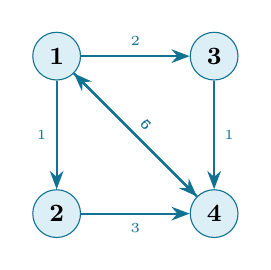
\begin{tikzpicture}[
        nd/.style={circle,draw=PrimaryMid,fill=PrimaryLight!50,
                   font=\bfseries\small,minimum size=0.6cm},
        arr/.style={-{Stealth},PrimaryMid,thick}
      ]
        \node[nd] (1) at (0,2) {1};
        \node[nd] (2) at (0,0) {2};
        \node[nd] (3) at (2,2) {3};
        \node[nd] (4) at (2,0) {4};
        \draw[arr] (1)--node[above,font=\tiny]{2}(3);
        \draw[arr] (1)--node[left,font=\tiny]{1}(2);
        \draw[arr] (2)--node[below,font=\tiny]{3}(4);
        \draw[arr] (3)--node[right,font=\tiny]{1}(4);
        \draw[arr] (4)--node[above,font=\tiny,sloped]{6}(1);
        \draw[arr] (1)--node[above,font=\tiny,sloped]{5}(4);
      \end{tikzpicture}
    \column{0.55\textwidth}
      \textbf{$D^{(0)}$ (initial):}
      \[
        \begin{pmatrix}
          0 & 1 & 2 & 5 \\
          \infty & 0 & \infty & 3 \\
          \infty & \infty & 0 & 1 \\
          6 & \infty & \infty & 0
        \end{pmatrix}
      \]
      \textbf{$D^{(4)}$ (final):}
      \[
        \begin{pmatrix}
          0 & 1 & 2 & 3 \\
          9 & 0 & 11 & 3 \\
          7 & 8 & 0 & 1 \\
          6 & 7 & 8 & 0
        \end{pmatrix}
      \]
      E.g., shortest path $2\to1 = 9$ (via $4\to1$, cost $3+6$).
  \end{columns}
\end{frame}

% ============================================================
\section{Coin-Collecting Problem}
% ============================================================

\begin{frame}[shrink=12]{Coin-Collecting on a Grid}
  \begin{columns}[T]
    \column{0.55\textwidth}
      \textbf{Problem:} A robot at cell $(1,1)$ collects coins while
      moving only \emph{right} or \emph{down} to reach $(n,m)$.
      Each cell has $c_{ij}$ coins.

      \vspace{0.3em}
      \textbf{Recurrence:}
      \[
        F(i,j) = \max\{F(i{-}1,j),\;F(i,j{-}1)\} + c_{ij}
      \]
      $F(0,j) = F(i,0) = 0$ (boundary)
    \column{0.40\textwidth}
      \textbf{Example ($5\times 6$ board):}
      \vspace{0.2em}

      \begin{tabular}{c*{6}{r}}
        \toprule
        & 1&2&3&4&5&6 \\
        \midrule
        1 & 0&0&0&0&1&1 \\
        2 & 0&1&1&2&2&2 \\
        3 & 0&1&1&3&3&4 \\
        4 & 0&1&2&3&3&5 \\
        5 & 1&1&2&3&4&\textbf{5} \\
        \bottomrule
      \end{tabular}
      \vspace{0.2em}
      Max coins = \highlight{5}\ctag{nm}
  \end{columns}
\end{frame}

% ── Chapter Summary ──────────────────────────────────────────
\begin{frame}[shrink=12]{Chapter 6 Summary}
  \begin{columns}[T]
    \column{0.55\textwidth}
      \textbf{Problems solved with DP:}
      \begin{tabular}{ll}
        \toprule
        Problem & Complexity \\
        \midrule
        Fibonacci    & $\Theta(n)$ \\
        Coin-Row     & $\Theta(n)$ \\
        Change-Making & $\mathcal{O}(nm)$ \\
        0-1 Knapsack & $\Theta(nW)$ \\
        Coin-Collecting & $\Theta(nm)$ \\
        Optimal BST  & $\Theta(n^3)$ \\
        Warshall / Floyd & $\Theta(n^3)$ \\
        \bottomrule
      \end{tabular}
    \column{0.40\textwidth}
      \begin{block}{DP recipe}
        \begin{enumerate}
          \item Define the sub-problem and its parameter(s)
          \item Write the recurrence (and base cases)
          \item Fill the DP table bottom-up (or use memoisation)
          \item Trace back to find the optimal solution
        \end{enumerate}
      \end{block}
      \vspace{0.2em}
      \begin{block}{Next chapter}
        \textbf{Chapter 7:} Greedy Algorithms — make
        locally optimal choices and prove global optimality.
      \end{block}
  \end{columns}
\end{frame}

\end{document}
